\documentclass[main.tex]{subfiles}
\begin{document}

\section{Voorbeelden in metrische ruimten}
\label{sec:voorb-metr-ruimt}


\subsection{De discrete metriek}
\label{sec:de-discrete-metriek}

\begin{vb}
  Zij $X$ een willekeurige, niet-lege verzameling.
  De \term{discrete metriek} of \term{triviale metriek} op $X$ wordt gegeven als volgt.
  \[
  d_{X}:\ X \times X \rightarrow \mathbb{R}^{+}:\ (x,y) \mapsto
  \begin{cases}
    0 &\text{ als } x = y\\
    1 &\text{ als } x \neq y
  \end{cases}
  \]
  $X,d_{X}$ vormt een metrische ruimte.
\end{vb}

\begin{st}
  Elke verzameling is begrensd voor de discrete metriek.

  \begin{proof}
    Inderdaad, de afstand tussen twee elementen is nooit groter dan $1$.
  \end{proof}
\end{st}

\begin{vb}
  Een open bol rond $x\in \mathbb{R}$ met straal $\delta\in \mathbb{R}_{0}^{+}$ voor de gewone metriek ziet eruit als volgt:
  \[ B(x,\delta) = 
  \begin{cases}
    \{x\} &\text{ als } r\le 1\\
    X &\text{ als } r > 1
  \end{cases}
  \]
\extra{bewijs}
\end{vb}

\begin{st}
  Elke deelverzameling $A$ van een verzameling $X$ is zowel open als gesloten voor de triviale metriek.
\extra{bewijs}
\end{st}


\begin{vb}
  Voor de triviale metriek $d_{X}$ voor een verzameling $X$, is elke functie $f:\ X \rightarrow Y$ met $Y,d_{Y}$ een metrische ruimte, continu.
\extra{bewijs}
\end{vb}

\begin{st}
  De triviale metriek $d_{X}$ voor een verzameling $X$ is topologisch fijner dan elke andere metriek op $X$.

  \begin{proof}
    De triviale topologie is de machtsverzameling $\mathcal{P}(X)$ van $X$.
    Omdat elke topologie een verzameling van deelverzamelingen van $X$ is, moet ze dus een deel zijn van $\mathcal{T}_{d_{X}}$.
  \end{proof}
\end{st}

\begin{st}
  Een deelverzameling $A$ van een willekeurige verzameling $X$ is zijn eigen sluiting en inwendige voor de triviale metriek.
\extra{bewijs}
\end{st}

\begin{st}
  Alle punten van een deelverzameling $A$ van een willekeurige verzameling $X$ zijn ge\"isoleerde punten voor de triviale metriek.
\extra{bewijs}
\end{st}

\begin{st}
  De verzameling $\{ x_{n} \mid n\in \mathbb{N} \}$ van elementen van een convergente rij $(x_{n})_{n}$ voor de discrete metriek is steeds eindig.

  \begin{proof}
    Zij $(x_{n})_{n}$ een convergente rij in een verzameling $X$ en noem $x$ de limiet..
    Omdat $(x_{n})_{n}$ convergeert, bestaat er een $n_{0}\in \mathbb{N}$ zodat alle $x_{n}$ vanaf $n_{0}$ dichter dan $1$ bij $x$ liggen en dus gelijk zijn aan $x$.
    Er zijn dan nog hoogstens $n_{0}-1$ (en dus hoogstens een eindig aantal) andere elementen in de rij te vinden.
  \end{proof}
\end{st}

\subsection{Metrieken op $\mathbb{R}$}
\label{sec:metrieken-op-mathbbr}

\subsubsection{De gewone metriek op $\mathbb{R}$}
\label{sec:de-gewone-metriek}

\begin{vb}
  $\mathbb{R}$, uitgerust met een metriek gebaseerd op de absolute-waardefunctie, is een metrische ruimte:
  \[ d:\ \mathbb{R}\times\mathbb{R}\rightarrow (x,y) \mapsto d(x,y)=|x-y| \]
  Men noemt dit de \term{gewone metriek op $\mathbb{R}$}.
\extra{bewijs}
\end{vb}

\begin{opm}
  $\mathbb{R}$ is niet begrensd voor $d$.
\extra{bewijs}
\end{opm}

\begin{vb}
  Een open bol rond $x\in \mathbb{R}$ met straal $\delta\in \mathbb{R}_{0}^{+}$ voor de gewone metriek ziet eruit als volgt:
  \[ B(x,\delta) = \interval[open]{x-\delta}{x+\delta} \]
  \begin{figure}[H]
    \centering
    \begin{tikzpicture}[scale=1.5]
      \draw[latex-latex] (-1.5,0) -- (1.5,0);
      \draw[color=black] (0pt,3pt) -- (0pt,-3pt) node[below] {$a$};
      \draw[(-),thick,color=red] (-1,0) -- (1,0);
    \end{tikzpicture}
    \caption{Een open bol in $\mathbb{R},d$}
  \end{figure}
\extra{bewijs}
\end{vb}

\begin{vb}
  $\mathbb{R},d$ is separabel door $\mathbb{Q}$.
\TODO{een echt bewijs dat $\mathbb{Q}$ dicht ligt in $\mathbb{R}$.}
\end{vb}

\begin{vb}
  De verzameling $\interval[open right]{0}{1}$ is niet compact.
  \begin{proof}
    Benoem $A = \interval[open right]{0}{1}$ en $\mathcal{F}$ als volgt:
    \[ \mathcal{F} = \left\{      \interval[open]{-1}{1-\frac{1}{n}} \mid n \in \mathbb{N}_{0} \right\} \]
    $\mathcal{F}$ is een verzameling van open delen van $\mathbb{R}$ en de unie ervan is $\interval[open]{0}{1}$, een oververzameling van $A$.
    $\mathcal{F}$ is dus een open overdekking van $A$.
    eze overdekking heeft geen eindige deeloverdekking.
    Elke deelverzameling van $\mathcal{F}$ is immers van de vorm $\interval[open]{-1}{1-\frac{1}{n}}$.
  \end{proof}
\end{vb}

\begin{vb}
  De verzameling $A$ als volgt is niet compact in $\mathbb{R},d$
  \[ A = \left\{ \frac{1}{n} \mid n\in \mathbb{N} \right\} \]

    \begin{proof}
      \noindent
      \begin{klad}
        We construeren een open overdekking $\mathcal{A}$ zodat elk element uit $A$ in hoogstens \'e\'en open deel in $\mathcal{A}$ zit.
        Beschouw eerst de afstand tussen twee opeenvolgende elementen uit $A$:
        \[ d\left(\frac{1}{n},\frac{1}{n+1}\right) = \frac{n+1 - n}{n(n+1)} = \frac{1}{n(n+1)} \]
        Als we rond elk element een open bol nemen met straal $r$ waarbij $r$ de helft is van de minimale afstand tussen twee elementen naast elkaar, dan hebben we een geschikte open overdekking.
      \end{klad}
      Beschouw de open overdekking $\mathcal{A}$ als volgt.
      \[ \left\{ B\left(\frac{1}{n},\frac{1}{2n(n+1)}\right) \mid n\in \mathbb{N} \right\} \]
      Merk op dat in elke open bol in $\mathcal{A}$ precies \'e\'en element van $A$ zit.
      Omdat $A$ oneindig veel elementen bevat heeft deze open overdekking dus geen eindige deeloverdekking.
    \end{proof}
\end{vb}

\begin{vb}
  De verzameling $B$ als volgt is compact in $\mathbb{R},d$.
  \[ B = \{0\} \cup \left\{ \frac{1}{n} \mid n\in \mathbb{N} \right\} \]

  \begin{proof}
    Kies een willekeurige overdekking $\mathcal{B}$ van $B$.
    We argumenteren dat $\mathcal{B}$ te reduceren valt tot een eindige deeloverdekking.
    \begin{klad}
      Omdat $0$ is $B$ zit, moet $0$ overdekt worden door een open deel.
      In dat open deel moeten oneindig veel elementen zitten uit $B$.
      Voor de overige elementen uit $B$ kiezen we dan nog een open deel uit $\mathcal{B}$ om onze eindige deeloverdekking te vervolledigen.
    \end{klad}
    Omdat $\mathcal{B}$ open is en $0$ bevat, bestaat er een $\delta \in \mathbb{R}_{0}^{+}$ zodat $B(0,\delta)$ een deelverzameling is van het open deel $O$ in $\mathcal{B}$ dat $0$ overdekt.
    Noem $m=\left\lceil\frac{1}{\delta}\right\rceil$ en merk dan op dat $B(0,\delta)$ alle elementen $\frac{1}{n}$ bevat met $n > m$.
    Kies nu nog voor elke $\frac{1}{n}$ met $n \le m$ een open deel $O_{n}$ uit $\mathcal{B}$ dat $\frac{1}{n}$ overdekt.
    Beschouw dan de open deeloverdekking $\{ O \} \cup \{ O_{n} \mid n \le m \}$.
    Deze deeloverdekking is eindig.
  \end{proof}
\end{vb}

\begin{vb}
  Een gesloten interval $\interval{a}{b}$ is compact in $\mathbb{R},d$.

  \begin{proof}
    Bewijs uit het ongerijmde:
    Stel dat er een open overdekking $\mathcal{O}$ van $\interval{0}{1}$ bestaat die geen eindige deeloverdekking heeft.
    Beschouw de twee helften $\interval{a}{\frac{a+b}{2}}$ en $\interval{\frac{a+b}{2}}{b}$.
    Minstens \'e\'en van de twee helften valt dan niet te eindig open de overdekken met een deel van $\mathcal{O}$.\waarom
    Noteer die helft met $\interval{a_{1}}{b_{1}}$
    We kunnen dit opnieuw blijven doen om een dalende rij intervallen $\left(\interval{a_{n}}{b_{n}}\right)_{n}$ te construeren die elk niet eindig te overdekken vallen met een deel van $\mathcal{O}$ en waarvan de lengte naar nul gaat.
    De doorsnede van al deze intervallen is een singleton, zeg $\{x\}$.\stref{st:geneste-intervallen}
    Neem nu een open deel $O$ in $\mathcal{O}$ dat $x$ overdekt.
    Omdat $O$ open is, bestaat er een $\delta \in \mathbb{R}_{0}^{+}$ zodat $B(x,\delta)$ een deel is van $O$.
    Voor $n$ voldoende groot \clarify{hoe groot?} zit $\interval{a_{n}}{b_{n}}$ dus volledig in $\mathcal{O}$.
    Dit is in strijd met de constructie van $\interval{a_{n}}{b_{n}}$.
    Contradictie.
  \end{proof}
\TODO{later makkelijker bewijzen via stelling ipv via definitie}
\end{vb}

\begin{vb}
  $\mathbb{Z}$ is niet compact in $\mathbb{R},d$.

  \begin{proof}
    Neem de open overdekking $\mathcal{F}$ als volgt:
    \[ \left\{ B\left(n,\frac{1}{2}\right) \mid n \in \mathbb{Z} \right\} \]
    Elk element van (het oneindige) $\mathbb{Z}$ zit in precies \'e\'en deelverzameling in $\mathcal{F}$.
    Er bestaat dus geen eindige deeloverdekking van $\mathcal{F}$.
  \end{proof}
\end{vb}

\begin{opm}
  In $\mathbb{R}^{p}$ kan je bovenstaand argument telkens gebruiken om te bewijzen dat een gesloten en begrensde verzameling compact is door de verzameling steeds op gelijkaardige wijze in $2^{p}$ te splitsen.
\end{opm}

\begin{vb}
  $\mathbb{R}_{0}$ is niet samenhangend.

  \begin{proof}
    Inderdaad, $\mathbb{R}_{0} = \mathbb{R}_{0}^{-} \cup \mathbb{R}_{0}^{+}$, $\overline{\mathbb{R}_{0}^{+}} \cap \mathbb{R}_{0}^{-} = \mathbb{R}^{+} \cap \mathbb{R}_{0}^{-} = \emptyset$ en $\overline{\mathbb{R}_{0}^{-}} \cap \mathbb{R}_{0}^{+} = \mathbb{R}^{-} \cap \mathbb{R}_{0}^{+} = \emptyset$ gelden. 
  \end{proof}
\end{vb}

\subsubsection{De $d_1$-metriek op $\mathbb{R}$}
\label{sec:d_1-metriek-op}

\begin{vb}
  $\mathbb{R}$, uitgerust met de volgende functie als metriek, is een metrische ruimte:
  \[ d_{1}:\ \mathbb{R}\times\mathbb{R}\rightarrow (x,y) \mapsto d_{1}(x,y)=\frac{|x-y|}{1+|x-y|} \]
  \begin{proof}
    We gaan elke eigenschap van een metrische ruimte na.
    \begin{itemize}
    \item $d$ is symmestrisch.
      Dit volgt meteen uit de symmetrie van de gewone metriek op $\mathbb{R}$.
    \item $d$ is nu als en slechts als de argumentien nul zijn.
      Dit volgt uit dezelfde eigenschap van de gewone metriek op $\mathbb{R}$
    \item $d$ voldoet aan de driehoeksongelijkheid:\\
      Kies $x,y,z \in \mathbb{R}$ en houdt de driehoeksongelijkheid voor de gewone metriek op $\mathbb{R}$ in het achterhoofd.
      Merk op dat de functie $f$ als volgt stijgend is.
      \[ f:\ \mathbb{R}^{+} \rightarrow \mathbb{R}^{+}:\ t \mapsto \frac{t}{1+t} \]
      \begin{align*}
        d_{1}(x,y)
        &= f(|x-y|)\\
        &\le f(|x-z|+|z-y|)\\
        &= \frac{|x-z|+|z-y|}{1+|x-z|+|z-y|}\\
        &= \frac{|x-z|}{1+|x-z|+|z-y|}+\frac{|z-y|}{1+|x-z|+|z-y|}\\
        &\le \frac{|x-z|}{1+|x-z|}+\frac{|z-y|}{1+|z-y|}\\
        &= d_{1}(x,z) + d_{1}(z,y)
      \end{align*}
    \end{itemize}
  \end{proof}
\end{vb}

\begin{st}
  Voor de $d_{1}$ metriek is $\mathbb{R}$ begrensd.
  \begin{proof}
    Kies willekeurig $x,y\in\mathbb{R}$ en kies $M=1\in \mathbb{R}^{+}$, dan geldt het volgende:
    \[ d_{1}(x,y) = \frac{|x-y|}{1+|x-y|} < M \]
  \end{proof}
\end{st}
\extra{vindt de diameter}

\begin{vb}
  Een open bol rond $x\in \mathbb{R}$ met straal $\delta\in \mathbb{R}_{0}^{+}$ voor de $d_{1}$-metriek ziet eruit als volgt:
  \[ B(x,\delta) = 
  \begin{cases}
    \mathbb{R} &\text{ als } r \ge 1\\
    \interval[open]{x-\frac{r}{1-r}}{x+\frac{r}{1-r}}
  \end{cases}
  \]
\extra{bewijs}
\end{vb}

\begin{st}
  Een deelverzameling $A$ van $\mathbb{R}$ is $d_{1}$-open als en slechts als ze open is voor de gewone metriek.
\extra{bewijs}
\end{st}

\subsubsection{De $d_2$-metriek op $\mathbb{R}$}
\label{sec:d_2-metriek-op}

\begin{vb}
  $\mathbb{R}$, uitgerust met de volgende functie als metriek, is een metrische ruimte:
  \[ d_{2}:\ \mathbb{R}\times\mathbb{R}\rightarrow (x,y) \mapsto d_{2}(x,y)=\left| \frac{x}{1+|x|} - \frac{y}{1+|y|} \right| \]
\extra{bewijs}
\end{vb}

\begin{st}
  Voor de $d_{2}$ metriek hierboven is $\mathbb{R}$ begrensd.
\extra{bewijs}
\end{st}
\extra{vindt de diameter}

\mst{Een deelverzameling $A$ van $\mathbb{R}$ is $d_{2}$-open als en slechts als ze open is voor de gewone metriek.}

\question{Hoe bewijzen we dat $d_{2}$ en $d$ topologisch equivalent zijn (lijkt evident) en hoe zien de open bollen eruit? (Die moeten toch assymmetrisch zijn...}

\begin{vb}
  $\mathbb{R},d_{2}$ en $\interval[open]{-1}{1},d$ zijn isometrisch.
\extra{bewijs} 
\end{vb}

\subsubsection{De $d_3$-metriek op $\mathbb{R}$}
\label{sec:d_3-metriek-op}

\begin{vb}
  De functie $d_{3}$ als volgt is een metriek voor $\mathbb{R}$.
  \[
  d_{3}:\ \mathbb{R} \times \mathbb{R} \rightarrow \mathbb{R}^{+}:\ (x,y) \mapsto
  \begin{cases}
    d_{3}(x,y) = |x-y| &\text{ als } x\neq 0 \neq y\\
    d_{3}(x,0) = d(0,x) = 1 + |x| &\text{ als } x \neq 0\\
    d_{3}(0,0) = 0
  \end{cases}
  \]

  \begin{proof}
    We gaan de eigenschappen van een metriek na.
    \begin{itemize}
    \item $d_{3}$ is symmetrisch. OK
    \item $d_{3}(x,y)$ is nul als en slechts als $x$ en $y$ nul zijn. OK
    \item Kies willekeurig drie getallen $x$, $y$, $z$.
      \[ d(x,z) \le d(x,y) + d(y,z) \]
      We moeten $8$ gevallen nagaan:
      \begin{enumerate}
      \item $x=0$, $y=0$, $z=0$: $d(0,0) = 0 \le 0 + 0 = d(0,0) + d(0,0)$. OK
      \item $x=0$, $y=0$, $z\neq0$: $d(0,z) = 1 + |z| \le 0 + 1 + |z| = d(0,0) + d(y,z)$. OK 
      \item $x=0$, $y=\neq$, $z=0$: $d(0,0) = 0 \le 1+|y| + 1+|y| = d(0,y) + d(y,0)$. OK
      \item $x=0$, $y\neq0$, $z\neq0$: $d(0,z) = 1+ |z| \le 1+|y| + |y-z| = d(0,y) + d(y,z)$. OK
      \item $x\neq0$, $y=0$, $z=0$: $d(x,0) = 1+|x| \le 1+|x| + 0 = d(x,0) + d(0,0)$. OK
      \item $x\neq0$, $y=0$, $z\neq0$: $d(x,z) = |x-z| \le 1+|x| + 1+|z| = d(x,0) + d(0,z)$. OK
      \item $x\neq0$, $y\neq0$, $z=0$: $d(x,0) = 1+|x| \le |x-y| + 1+|y| = d(x,y) + d(y,0)$. OK
      \item $x\neq0$, $y\neq0$, $z\neq0$: $d(x,z) = |x-z| \le |x-y| + |y-z| = d(x,y) + d(y,z)$. OK
      \end{enumerate}
    \end{itemize}
  \end{proof}
\end{vb}


\subsection{Metrieken op $\mathbb{R}^p$}
\label{sec:metr-op-mathbbrp}

\subsubsection{De gewone metriek op $\mathbb{R}^p$}
\label{sec:gewone-metriek-op}

\begin{vb}
  $\mathbb{R}^{p}$, uitgerust met de volgende functie als metriek, is een metrische ruimte:
  \[ d:\ \mathbb{R}^{p}\times\mathbb{R}^{p}\rightarrow (x,y) \mapsto d(x,y)=\|x-y\| \]
  We noemen dit de \term{gewone metriek} of \term{euclidische metriek} op $\mathbb{R}^{p}$.
  \extra{bewijs}
  \begin{figure}[H]
    \centering
    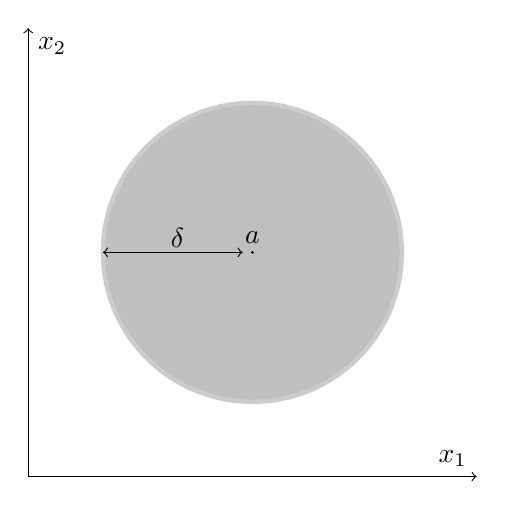
\begin{tikzpicture}
      \begin{axis}[ 
        ticks=none,
        axis lines = middle,
        axis line style={->},
        ymin=0, ymax=3,
        xmin=0, xmax=3,
        xlabel={$x_{1}$},
        ylabel={$x_{2}$},
        axis equal image,
        disabledatascaling
        ]
        \filldraw [ultra thick,fill=black!25!white, draw=black!20!white] (1.5,1.5) circle [radius=1];
        \fill [fill=black] (1.5,1.5) circle [radius=0.01];
        \draw (1.5,1.6) node {$a$};
        \draw (1.5,1.5) node {} edge[<->] (0.5,1.5);
        \draw (1,1.6) node {$\delta$};
      \end{axis}
    \end{tikzpicture}
    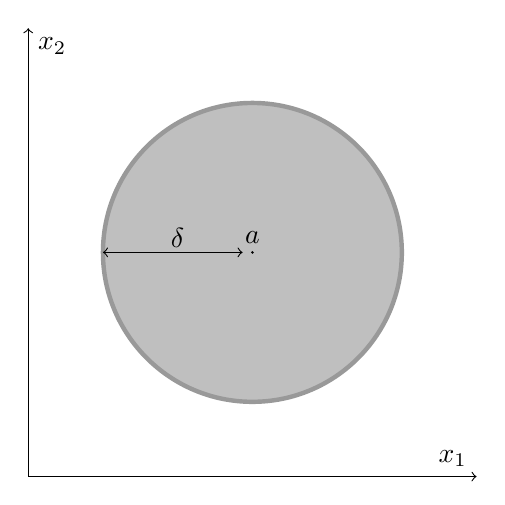
\begin{tikzpicture}
      \begin{axis}[ 
        ticks=none,
        axis lines = middle,
        axis line style={->},
        ymin=0, ymax=3,
        xmin=0, xmax=3,
        xlabel={$x_{1}$},
        ylabel={$x_{2}$},
        axis equal image,
        disabledatascaling
        ]
        \filldraw [ultra thick,fill=black!25!white, draw=black!40!white] (1.5,1.5) circle [radius=1];
        \fill [fill=black] (1.5,1.5) circle [radius=0.01];
        \draw (1.5,1.6) node {$a$};
        \draw (1.5,1.5) node {} edge[<->] (0.5,1.5);
        \draw (1,1.6) node {$\delta$};
      \end{axis}
    \end{tikzpicture}
    \caption{Een open bol en een gesloten bol in $\mathbb{R}^{2},d$}
  \end{figure}
\end{vb}

\begin{vb}
  $\mathbb{R}^{p},d$ is separabel door $\mathbb{Q}^{p}$.
\extra{bewijs}
\end{vb}

\begin{st}
  \examenvraag{TTT II 2014}
  Zij $A$ en $B$ twee niet-lege, onderling disjuncte delen van $\mathbb{R}^{p}$ met $p \ge 2$ en benoem $\delta$ als volgt:
  \[ \delta = \inf \{ \|a-b\| \mid a\in A, b\in B \} \]
  \begin{enumerate}
  \item Als $A$ en $B$ beide gesloten en begrensd zijn, geldt $\delta > 0$.
  \item Geef expliciete tegenvoorbeelden als \'e\'en van de voorwaarden niet geldt.
  \item Argumenteer of dit resultaat valt te verheffen naar willekeurige metrische ruimten.
  \end{enumerate}

  \begin{klad}
    Allereerst moeten we een idee krijgen van wat $\delta$ precies voorstelt.
    Het ziet ernaar uit dat $\delta$ voorstelt wat we de ``afstand'' tussen twee vlakke figuren zouden noemen.
    Intu\"itief kennen we natuurlijk enkel de afstand voor wat we ``normale'' figuren zouden noemen.
  \end{klad}

  \begin{enumerate}
  \item
    \begin{klad}
      Intu\"itief: De verzameling $V = \{ \|a-b\| \mid a \in A, b \in B \}$ zal gesloten en (naar onder) begrensd zijn als zowel $A$ als $B$ begrensd is.
      Van een gesloten en begrensde verzameling weten we dat het infimum erin zit.
      Omdat de verzamelingen $A$ en $B$ disjunct zijn, kan $0$ geen element zijn in die verzameling $V$.
    \end{klad}
    \begin{proof}
      Bewijs uit het ongerijmde: stel dat $\delta$ niet strikt positief is.\\
      Strikt negatief kan $\delta$ niet zijn, want normen zijn positief.
      Stel daarom dat $\delta$ nul is.
      Omdat $V$ een begrensde verzameling is, bestaat het infimum.
      Het infimum is dan een element van $\overline{V}$\waarom
      \TODO{het infimum van een begrensde verzameling behoort tot de sluiting ervan}
      Omdat $\delta$ tot $\overline{V}$ behoort, bestaat er een rij $(z_{n})_{n}$ in $V$ die naar $\delta$ convergeert.\prref{pr:metrische-ruimte-sluiting-itv-limiet}
      De rij $(z_{n})_{n}$ kunnen we beschrijven als $(\|a_{n}-b_{n}\|)_{n}$ met $(a_{n})_{n}$ en $(b_{n})_{n}$ respectievelijk rijen in $A$ en $B$.
      Omdat $A$ en $B$ gesloten en begrensd zijn, bestaan er een convergente deelrijen $(a_{n_{k}})_{k}$ en $(b_{n_{k}})_{k}$ van respectievelijk $(a_{n})_{n}$ en $(b_{n})_{n}$.\stref{st:in-rp-gesloten-en-begrensd-itv-rijen}
      Noem $a$ en $b$ de respectievelijke limieten van deze deelrijen.
      De limiet van $(\|a_{n_{k}}-b_{n_{k}}\|)_{k}$ is dan $|a-b|$.\waarom
      Dit is bovendien ook de limiet van $(\|a_{n}-b_{n}\|)_{n}$.\stref{st:in-rp-deelrij-zelfde-limiet}
      Omdat $|a-b|$ nul is, moeten $a$ en $b$ gelijk zijn.\deref{de:norm}
      Dit is in tegenspraak met de disjunctheid van $A$ en $B$.
      Contradictie.
    \end{proof}
  \item
    \begin{itemize}
    \item Als $A$ en $B$ niet begrensd zijn (maar wel gesloten) kan $\delta$ nul zijn.
      \begin{proof}
        Kies $A$ en $B$ als volgt:

        \noindent
        \begin{minipage}{.45\textwidth}
          \begin{figure}[H]
            \centering
            \begin{tikzpicture}
              \begin{axis}[ 
                ticks=none,
                axis lines = middle,
                axis line style={->},
                ymin=-3, ymax=3,
                xmin=0, xmax=10,
                xlabel={$x_{1}$},
                ylabel={$x_{2}$},
                axis equal image,
                disabledatascaling
                ]
                \addplot[name path=A1,color=red,thick,domain=0.1:9]{1/x};
                \addplot[name path=A2,color=white,domain=0.1:9]{3};
                \addplot[red!20] fill between[of=A1 and A2];
                \addplot[name path=B1,color=blue,thick,domain=0.1:9]{-1/x};
                \addplot[name path=B2,color=white,domain=0.1:9]{-3};
                \addplot[blue!20] fill between[of=B1 and B2];
                
                \draw (1.5,1.5) node {$A$};
                \draw (1.5,-1.5) node {$B$};
              \end{axis}
            \end{tikzpicture}
          \end{figure}
        \end{minipage}
        \begin{minipage}{.45\textwidth}
          \[ A = \left\{ \left(r,+q\right) \ \middle|\  r \in \mathbb{R}_{0}^{+}, q\in \mathbb{R}_{0}^{+}: q \ge r \right\} \]
          \[ B = \left\{ \left(r,-q\right) \ \middle|\  r \in \mathbb{R}_{0}^{+}, q\in \mathbb{R}_{0}^{+}: q \ge r \right\} \]
        \end{minipage}

        Het is duidelijk dat $A$ en $B$ beide niet begrensd zijn, maar wel gesloten.
        $\delta$ is toch $0$:
        \[ \delta = \inf \{ \|a-b\| \mid a \in A, b \in B \} = \inf \interval[open]{0}{+\infty} = 0\]
      \end{proof}
    \item Als $A$ en $B$ niet gesloten zijn (maar wel begrensd) kan $\delta$ nul zijn.
      \begin{proof}
        Kies $A$ en $B$ als volgt:

        \noindent
        \begin{minipage}{.45\textwidth}
          \begin{figure}[H]
            \centering
            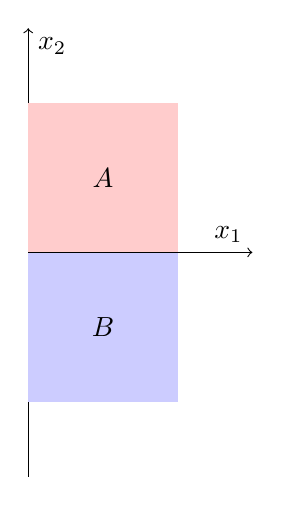
\begin{tikzpicture}
              \begin{axis}[ 
                ticks=none,
                axis lines = middle,
                axis line style={->},
                ymin=-1.5, ymax=1.5,
                xmin=0, xmax=1.5,
                xlabel={$x_{1}$},
                ylabel={$x_{2}$},
                axis equal image,
                disabledatascaling
                ]
                \fill [color=red!20] (0.0,0.001) rectangle (1,1);
                \fill [color=blue!20] (0.0,-0.001) rectangle (1,-1);
                \draw (0.5,0.5) node {$A$};
                \draw (0.5,-0.5) node {$B$};
              \end{axis}
            \end{tikzpicture}
          \end{figure}
        \end{minipage}
        \begin{minipage}{.45\textwidth}
          \[ A = \left\{ (x,+y) \mid x \in \interval[open]{0}{1} \wedge y\in \interval[open]{0}{1} \right\} \]
          \[ A = \left\{ (x,-y) \mid x \in \interval[open]{0}{1} \wedge y\in \interval[open]{0}{1} \right\} \]
        \end{minipage}
        
        Het is duidelijk dat $A$ en $B$ beide niet gesloten zijn, maar wel begrensd.
        $\delta$ is toch $0$:
        \[ \delta = \inf \{ \|a-b\| \mid a \in A, b \in B \} = \inf \interval[open]{0}{\sqrt{5}} \]
      \end{proof}
    \end{itemize}
  \item In willekeurige metrische ruimten bestaat er geen norm, maar we kunnen de stelling herformuleren als volgt:
    Zij $A$ en $B$ twee niet-lege, onderling disjuncte delen van een metrische ruimte $X,d$ en benoem $\delta$ als volgt:
    \[ \delta = \inf \{ d(a,b) \mid a\in A, b\in B \} \]
    Zelfs dan gaat de bewering niet op:
    \begin{proof}
      Beschouw de verzamelingen $A = \{ F_{2n} \mid n \in \mathbb{N}_{0} \}$ en $B = \{ F_{2n+1} \mid n\in \mathbb{N}_{0} \}$ in de metrische ruimte $\mathcal{F},h$ (uit voorbeeld \ref{vb:ttt-2-2014-1} op pagina \pageref{vb:ttt-2-2014-1}) 
      $A$ en $B$ zijn disjunct, begrensd en gesloten, maar $\delta$ zal toch $0$ zijn.
    \end{proof}
  \item Neem in plaats van $\mathbb{R}^{p}$ een willekeurige genormeerde vectorruimte en definieer de afstandsfunctie aan de hand van de norm.
    \extra{In een willekeurige genormeerde ruimte lijkt de stelling wel te gelden, bewijs}
  \end{enumerate}
  \feed
\end{st}

\subsubsection{De $d_1$- of city block metriek op $\mathbb{R}^p$}
\label{sec:de-d_1-city}

\begin{vb}
  $\mathbb{R}^{p}$, uitgerust met de volgende functie als metriek, is een metrische ruimte:
  \[ d_{1}:\ \mathbb{R}^{p}\times\mathbb{R}^{p}\rightarrow (x,y) \mapsto d_{1}(x,y)=\sum_{i=1}^{p}|x_{i}-y_{i}| \]
  We noemen dit de \term{city block metriek} of \term{taxicab metriek}.
\extra{bewijs}
  \begin{figure}[H]
    \centering
    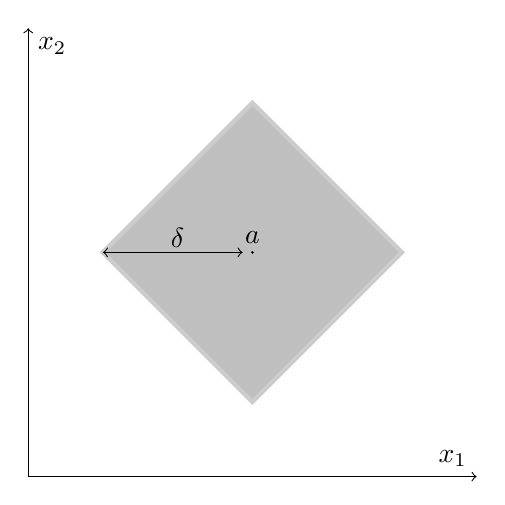
\begin{tikzpicture}
      \begin{axis}[ 
        ticks=none,
        axis lines = middle,
        axis line style={->},
        ymin=0, ymax=3,
        xmin=0, xmax=3,
        xlabel={$x_{1}$},
        ylabel={$x_{2}$},
        axis equal image,
        disabledatascaling
        ]
        \filldraw[ultra thick,fill=black!25!white, draw=black!20!white] (0.5,1.5) -- (1.5,2.5) -- (2.5,1.5) -- (1.5,0.5) -- cycle;
        \fill [fill=black] (1.5,1.5) circle [radius=0.01];
        \draw (1.5,1.6) node {$a$};
        \draw (1.5,1.5) node {} edge[<->] (0.5,1.5);
        \draw (1,1.6) node {$\delta$};
      \end{axis}
    \end{tikzpicture}
    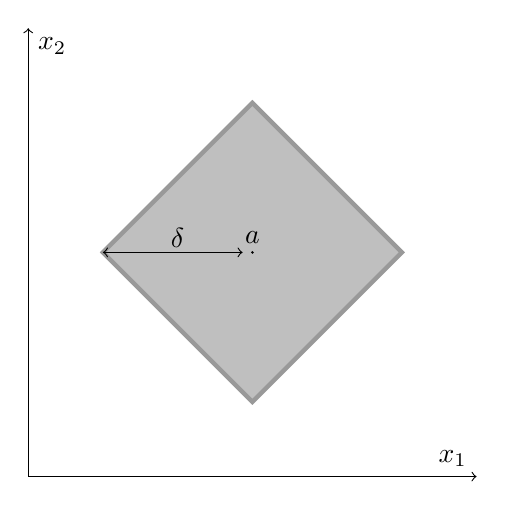
\begin{tikzpicture}
      \begin{axis}[ 
        ticks=none,
        axis lines = middle,
        axis line style={->},
        ymin=0, ymax=3,
        xmin=0, xmax=3,
        xlabel={$x_{1}$},
        ylabel={$x_{2}$},
        axis equal image,
        disabledatascaling
        ]
        \filldraw[ultra thick,fill=black!25!white, draw=black!40!white] (0.5,1.5) -- (1.5,2.5) -- (2.5,1.5) -- (1.5,0.5) -- cycle;
        \fill [fill=black] (1.5,1.5) circle [radius=0.01];
        \draw (1.5,1.6) node {$a$};
        \draw (1.5,1.5) node {} edge[<->] (0.5,1.5);
        \draw (1,1.6) node {$\delta$};
      \end{axis}
    \end{tikzpicture}
    \caption{Een open bol en een gesloten bol in $\mathbb{R}^{2},d_{1}$}
  \end{figure}
\end{vb}

\begin{st}
  $d$ en $d_{1}$ zijn topologisch equivalent op $\mathbb{R}^{p}$.

  \begin{proof}
    We moeten bewijzen dat er voor elke open bol $B(x,r)$ voor de gewone metriek een $d_{1}$-open bol $B_{1}(x,r_{1})$ bestaat met hetzelfde middelpunt die erin ligt en omgekeerd.
    \begin{itemize}
    \item $\Rightarrow$\\
      Kies een open bol $B(x,r)$ voor de gewone metriek.
      $B_{1}(x,r)$ voor de $d_{1}$ metriek is er dan een deel van:
      \[ \forall x,y\in A:\ d_{1}(x,y)^{2} = \left(\sum_{i=1}^{p}|x_{i}-y_{i}|\right)^{2} \ge \sum_{i=1}^{p}|x_{i}-y_{i}| = d(x,y)^{2} \]
      Als $d_{1}(x,y)$ dus kleiner is dan $r$ dan zal $d(x,y)$ dat ook zijn.

      \begin{figure}[H]
        \centering
        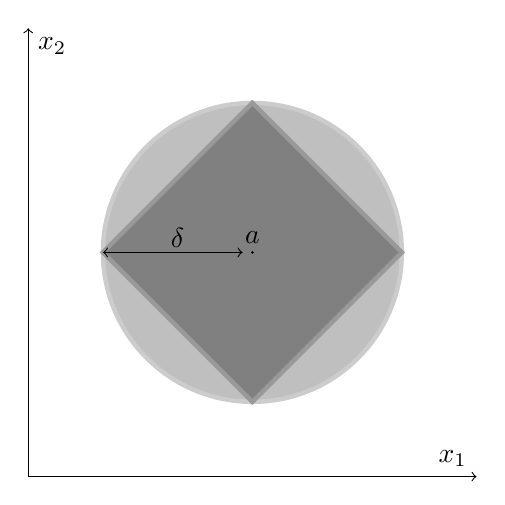
\begin{tikzpicture}
          \begin{axis}[ 
            ticks=none,
            axis lines = middle,
            axis line style={->},
            ymin=0, ymax=3,
            xmin=0, xmax=3,
            xlabel={$x_{1}$},
            ylabel={$x_{2}$},
            axis equal image,
            disabledatascaling
            ]
            \filldraw [ultra thick,fill=black!25!white, draw=black!20!white] (1.5,1.5) circle [radius=1];
            \filldraw[ultra thick,fill=black!50!white, draw=black!40!white] (0.5,1.5) -- (1.5,2.5) -- (2.5,1.5) -- (1.5,0.5) -- cycle;
            \fill [fill=black] (1.5,1.5) circle [radius=0.01];
            \draw (1.5,1.6) node {$a$};
            \draw (1.5,1.5) node {} edge[<->] (0.5,1.5);
            \draw (1,1.6) node {$\delta$};
          \end{axis}
        \end{tikzpicture}
        \caption{Een illustratie in $\mathbb{R}^{2}$}
      \end{figure}

    \item $\Leftarrow$\\
      Omgekeerd moeten we voor $r_{1}$ eenvoudigweg $\frac{r}{\sqrt{p}}$ nemen:
      \[ \forall x,y \in A:\ B_{1}(x,r) = \sum_{i=1}^{p}|x_{i}-y_{i}| \le \sqrt{\sum_{i=1}^{p}1} \sqrt{\sum_{i=1}^{p}|x_{i}-y_{i}|} = \sqrt{p}d(x,y) \]

      \begin{figure}[H]
        \centering
        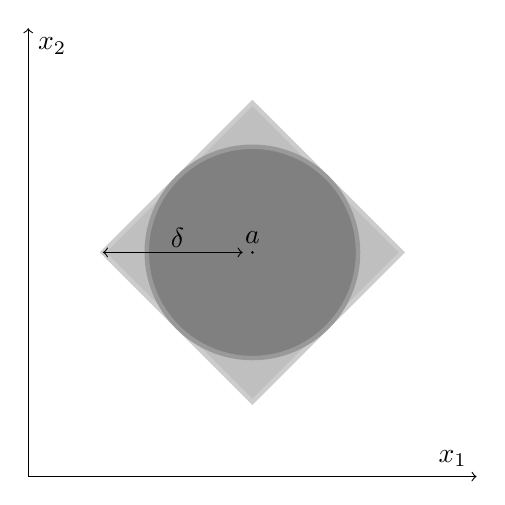
\begin{tikzpicture}
          \begin{axis}[ 
            ticks=none,
            axis lines = middle,
            axis line style={->},
            ymin=0, ymax=3,
            xmin=0, xmax=3,
            xlabel={$x_{1}$},
            ylabel={$x_{2}$},
            axis equal image,
            disabledatascaling
            ]
            \filldraw[ultra thick,fill=black!25!white, draw=black!20!white] (0.5,1.5) -- (1.5,2.5) -- (2.5,1.5) -- (1.5,0.5) -- cycle;
            \filldraw [ultra thick,fill=black!50!white, draw=black!40!white] (1.5,1.5) circle [radius=1/sqrt(2)];
            \fill [fill=black] (1.5,1.5) circle [radius=0.01];
            \draw (1.5,1.6) node {$a$};
            \draw (1.5,1.5) node {} edge[<->] (0.5,1.5);
            \draw (1,1.6) node {$\delta$};
          \end{axis}
        \end{tikzpicture}
        \caption{Een illustratie in $\mathbb{R}^{2}$}
      \end{figure}
    \end{itemize}
  \end{proof}
\end{st}

\subsubsection{De $d_\infty$- of maximummetriek op $\mathbb{R}^p$}
\label{sec:de-d_infty-maxim}

\begin{vb}
  $\mathbb{R}^{p}$, uitgerust met de volgende functie als metriek, is een metrische ruimte:
  \[ d_{\infty}:\ \mathbb{R}^{p}\times\mathbb{R}^{p}\rightarrow (x,y) \mapsto d_{\infty}(x,y)=\max_{i}|x_{i}-y_{i}| \]
  We noemen dit de \term{maximummetriek}.
\extra{bewijs}
  \begin{figure}[H]
    \centering
    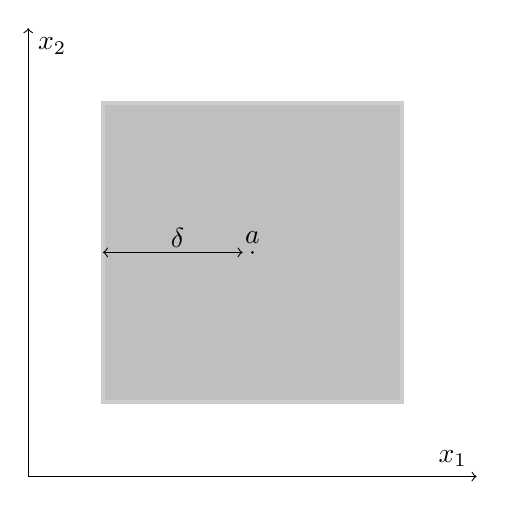
\begin{tikzpicture}
      \begin{axis}[ 
        ticks=none,
        axis lines = middle,
        axis line style={->},
        ymin=0, ymax=3,
        xmin=0, xmax=3,
        xlabel={$x_{1}$},
        ylabel={$x_{2}$},
        axis equal image,
        disabledatascaling
        ]
        \filldraw[ultra thick,fill=black!25!white, draw=black!20!white] (0.5,2.5) -- (2.5,2.5) -- (2.5,0.5) -- (0.5,0.5) -- cycle;
        \fill [fill=black] (1.5,1.5) circle [radius=0.01];
        \draw (1.5,1.6) node {$a$};
        \draw (1.5,1.5) node {} edge[<->] (0.5,1.5);
        \draw (1,1.6) node {$\delta$};
      \end{axis}
    \end{tikzpicture}
    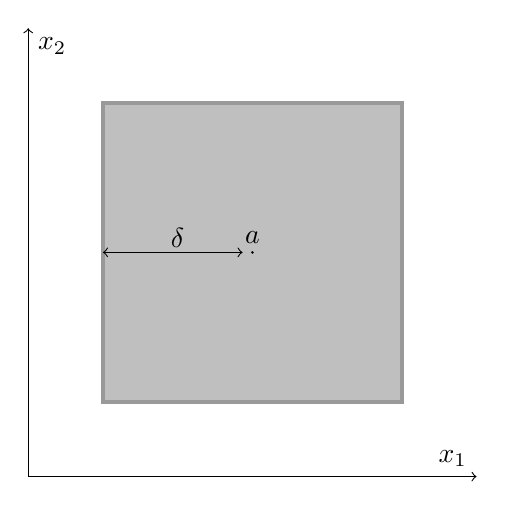
\begin{tikzpicture}
      \begin{axis}[ 
        ticks=none,
        axis lines = middle,
        axis line style={->},
        ymin=0, ymax=3,
        xmin=0, xmax=3,
        xlabel={$x_{1}$},
        ylabel={$x_{2}$},
        axis equal image,
        disabledatascaling
        ]
        \filldraw[ultra thick,fill=black!25!white, draw=black!40!white] (0.5,2.5) -- (2.5,2.5) -- (2.5,0.5) -- (0.5,0.5) -- cycle;
        \fill [fill=black] (1.5,1.5) circle [radius=0.01];
        \draw (1.5,1.6) node {$a$};
        \draw (1.5,1.5) node {} edge[<->] (0.5,1.5);
        \draw (1,1.6) node {$\delta$};
      \end{axis}
    \end{tikzpicture}
    \caption{Een open bol en een gesloten bol in $\mathbb{R}^{2},d_{\infty}$}
  \end{figure}
\end{vb}

\begin{st}
  $d$ en $d_{1}$ zijn topologisch equivalent op $\mathbb{R}^{p}$.

  \begin{proof}
    We moeten bewijzen dat er voor elke open bol $B(x,r)$ voor de gewone metriek een $d_{\infty}$-open bol $B_{\infty}(x,r_{1})$ bestaat met hetzelfde middelpunt die erin ligt en omgekeerd.
    \begin{itemize}
    \item $\Leftarrow$\\
      Kies $r_{\infty} = \frac{1}{\sqrt{p}}r$:
      \extra{bewijs}

      \begin{figure}[H]
        \centering
        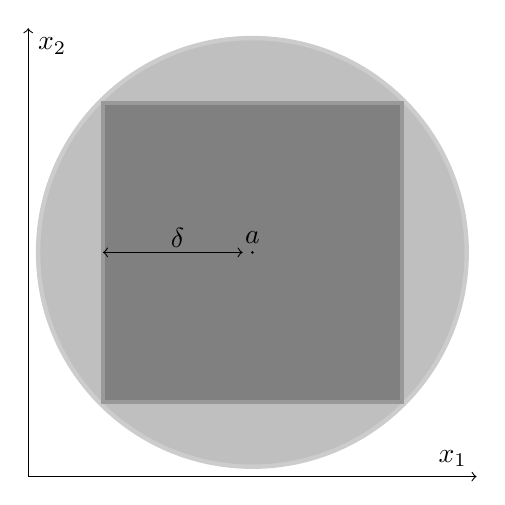
\begin{tikzpicture}
          \begin{axis}[ 
            ticks=none,
            axis lines = middle,
            axis line style={->},
            ymin=0, ymax=3,
            xmin=0, xmax=3,
            xlabel={$x_{1}$},
            ylabel={$x_{2}$},
            axis equal image,
            disabledatascaling
            ]
            \filldraw [ultra thick,fill=black!25!white, draw=black!20!white] (1.5,1.5) circle [radius=sqrt(2)+0.02];
            \filldraw[ultra thick,fill=black!50!white, draw=black!40!white] (0.5,2.5) -- (2.5,2.5) -- (2.5,0.5) -- (0.5,0.5) -- cycle;
            \fill [fill=black] (1.5,1.5) circle [radius=0.01];
            \draw (1.5,1.6) node {$a$};
            \draw (1.5,1.5) node {} edge[<->] (0.5,1.5);
            \draw (1,1.6) node {$\delta$};
          \end{axis}
        \end{tikzpicture}
        \caption{Een illustratie in $\mathbb{R}^{2}$}
      \end{figure}

    \item $\Rightarrow$\\
      Kies $r = r_{\infty}$:
      \extra{bewijs}

      \begin{figure}[H]
        \centering
        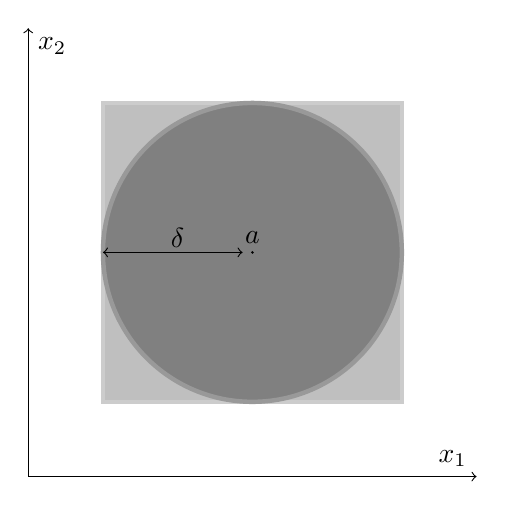
\begin{tikzpicture}
          \begin{axis}[ 
            ticks=none,
            axis lines = middle,
            axis line style={->},
            ymin=0, ymax=3,
            xmin=0, xmax=3,
            xlabel={$x_{1}$},
            ylabel={$x_{2}$},
            axis equal image,
            disabledatascaling
            ]
            \filldraw[ultra thick,fill=black!25!white, draw=black!20!white] (0.5,2.5) -- (2.5,2.5) -- (2.5,0.5) -- (0.5,0.5) -- cycle;
            \filldraw [ultra thick,fill=black!50!white, draw=black!40!white] (1.5,1.5) circle [radius=1];
            \fill [fill=black] (1.5,1.5) circle [radius=0.01];
            \draw (1.5,1.6) node {$a$};
            \draw (1.5,1.5) node {} edge[<->] (0.5,1.5);
            \draw (1,1.6) node {$\delta$};
          \end{axis}
        \end{tikzpicture}
        \caption{Een illustratie in $\mathbb{R}^{2}$}
      \end{figure}

    \end{itemize}
  \end{proof}
\end{st}

\subsubsection{De spoorwegmetriek op $\mathbb{R}^p$}
\label{sec:de-spoorw-op}

\begin{vb}
  $\mathbb{R}^{p}$, uitgerust met de volgende functie als metriek, is een metrische ruimte:
  \[
  d_{NMBS}:\ \mathbb{R}^{p}\times\mathbb{R}^{p}\rightarrow (x,y) \mapsto d_{NMBS}(x,y)=
  \begin{cases}
    \|x-y\| &\text{ als $x$ en $y$ lineair afhankelijk zijn}\\
    \|x\|+\|y\| &\text{ als $x$ en $y$ lineair onafhankelijk zijn}
  \end{cases}
  \]
  We noemen dit de \term{spoorwegmetriek}.
\extra{bewijs}
  \begin{figure}[H]
    \centering
    \begin{tikzpicture}
      \begin{axis}[ 
        ticks=none,
        axis lines = middle,
        axis line style={->},
        ymin=-1.5, ymax=2.5,
        xmin=-1.5, xmax=2.5,
        xlabel={$x_{1}$},
        ylabel={$x_{2}$},
        axis equal image,
        disabledatascaling
        ]
        \filldraw [ultra thick,fill=black!25!white, draw=black!20!white] (0,0) circle [radius=0.5];
        \fill [fill=black] (0.55,0.1) circle [radius=0.02];
        \draw [(-,color=black] (1.65,0.3) -- (0,0);
        \draw (0.55,0.2) node {$a$};
      \end{axis}
    \end{tikzpicture}
    \begin{tikzpicture}
      \begin{axis}[ 
        ticks=none,
        axis lines = middle,
        axis line style={->},
        ymin=0, ymax=2.5,
        xmin=0, xmax=2.5,
        xlabel={$x_{1}$},
        ylabel={$x_{2}$},
        axis equal image,
        disabledatascaling
        ]
        \fill [fill=black] (1.0,0.5) circle [radius=0.01];
        \draw [(-),color=black] (0.5,0.25) -- (1.5,0.75);
        \draw (1.1,0.4) node {$a$};
      \end{axis}
    \end{tikzpicture}
    \caption{Twee open bollen in $\mathbb{R}^{2},d_{NMBS}$ van verschillende straal}
  \end{figure}
\end{vb}

\subsection{Metrieken op rijruimten}
\label{sec:metr-op-rijr}

\begin{de}
  We noteren met $\mathbb{R}^{\mathbb{N}}$ de verzamelingen van alle rijen in $\mathbb{R}$.
  Merk op dat $\mathbb{R}^{\mathbb{N}}$ een vectorruimte is over $\mathbb{R}$.
\end{de}

\subsubsection{Een metriek op de hele rijruimte van $\mathbb{R}$}
\label{sec:een-metriek-op}

\begin{vb}
  $\mathbb{R}^{\mathbb{N}}$, uitgerust met de volgende functie als metriek, is een metrische ruimte:
  \[ d:\ \mathbb{R}^{\mathbb{N}} \times \mathbb{R}^{\mathbb{N}} \rightarrow \mathbb{R}^{+}:\ ((x_{n})_{n},(y_{n})_{n}) \mapsto \sum_{n=0}^{+\infty}\frac{|x_{n}-y_{n}|}{2^{n}(1+|x_{n}-y_{n}|)} \]
\extra{bewijs en bewijs waarom dit goed gedefinieerd is}
\end{vb}

\subsubsection{Een metriek op de begrensde rijen in $\mathbb{R}$}
\label{sec:een-metriek-op-1}

\begin{vb}
  Noteer met $l^{\infty}(\mathbb{N})$ het volgende:
  \[ l^{\infty}(\mathbb{N}) = \{ (x_{n})_{n} \in \mathbb{R}^{\mathbb{N}} \mid (x_{n})_{n} \text{ is begrensd.}\} \]
  $l^{\infty}$, uitgerust met de volgende functie als metriek, is een metrische ruimte:
  \[ d_{\infty}:\ \mathbb{R}^{\mathbb{N}} \times \mathbb{R}^{\mathbb{N}} \rightarrow \mathbb{R}^{+}:\ ((x_{n})_{n},(y_{n})_{n}) \mapsto \sup\{|x_{n}-y_{n}| \mid n\in \mathbb{N}\} \]
\extra{bewijs}
\end{vb}

\begin{vb}
  De metrische ruimte $l^{\infty},d_{\infty}$ is niet separabel.
  
  \begin{proof}
    Bewijs uit het ongerijmde: Stel dat er een deel $Q$ van $l^{\infty}(\mathbb{N})$ bestaat dat dicht ligt in $l^{\infty}(\mathbb{N}),Q$.\\
    Beschouw de verzameling $A$ als volgt:
    \[ A = \{ (x_{n})_{n} \in l^{\infty}(\mathbb{N}) \mid \forall n\in \mathbb{N}:\ x_{n} \in \{0,1\} \]
    Merk op dat de $d_{\infty}$ afstand tussen elke twee verschillende rijen in $A$ gelijk is aan $1$ en dat $A$ niet aftelbaar is.\waarom
    Voor elke $x\in A$ kunnen we dan een $q_{x}\in Q$ vinden zodat $d_{\infty}(x,q_{x})$ kleiner is dan $\frac{1}{2}$.
    Voor twee verschillende $x,y\in A$ moet $q_{x}$ bovendien verschillend zijn van $q_{y}$:
    \[ 1 = d_{\infty}(x,y) \le d_{\infty}(x,q_{x}) + d_{\infty}(q_{x},q_{y}) + d_{\infty}(q_{y},y) < \frac{1}{2} + d_{\infty}(q_{x},q_{y}) + \frac{1}{2} \]
    Het dicht deel $Q$ bevat dus een niet aftelbare deelverzameling, namelijk $\{q_{x} \mid x\in A\}$, en kan dus niet aftelbaar zijn.
    \extra{meer uitleg over het idee hiervan}
  \end{proof}
\end{vb}

\subsubsection{Een metriek op de absoluut convergente reeksen in $\mathbb{R}$}
\label{sec:een-metriek-op-2}

\begin{vb}
  Noteer met $l^{1}(\mathbb{N})$ de verzameling van absoluut convergente reeksen in $\mathbb{R}$:
  \[ l^{1}(\mathbb{N}) = \left\{ (x_{n})_{n} \ \middle|\ \sum_{n}|x_{n}| \right\} \]
  Deze verzameling, uitgerust met de volgende functie als metriek, vormt een metrische ruimte.
  \[ d_{1}:\ l^{1}(\mathbb{N}) \times l^{1}(\mathbb{N}) \rightarrow \mathbb{R}^{+}:\ d_{1}((x_{n})_{n},(y_{n})_{n}) = \sum_{n}|x_{n}-y_{n}| \]
\extra{bewijs}
\end{vb}

\begin{vb}
  De metrische ruimte $l^{1}(\mathbb{N}),d_{1}$ is separabel.
  
  \begin{proof}
    Beschouw de verzameling van rijen van rationale getallen die eindigen met een staart van nullen:
    \[ Q = \{ (q_{n})_{n} \in l^{1}(\mathbb{N}) \mid \forall n\in \mathbb{N}:\ q_{n}\in \mathbb{Q} \wedge \exists n_{0}\in \mathbb{N}, \forall n\in \mathbb{N}:\ n \ge n_{0} \Rightarrow q_{n} = 0 \} \]
    Merk op dat $Q$ aftelbaar is.
    $Q$ ligt bovendien dicht in $l^{1}(\mathbb{N})$:
    Kies immers een willekeurige $(x_{n})_{n}\in l^{1}(\mathbb{N})$ en een willekeurige $\epsilon \in \mathbb{R}_{0}^{+}$.
    We tonen aan dat er een $q\in Q$ bestaat zodat $d_{1}((x_{n})_{n},q)$ kleiner is dan $\epsilon$.\stref{st:metrische-ruimte-dicht-in-test}
    Kies eerst $n_{0}\in \mathbb{N}$ als volgt:
    \[ \sum_{n=n_{0}+1}^{\infty}|x_{n}| < \frac{\epsilon}{2} \]
    Kies vervolgens $n_{0}+1$ rationale getallen $r_{n}\in \mathbb{Q}$ als volgt:
    \[ |x_{n}-r_{n}| < \frac{\epsilon}{2^{n+2}} \]
    Stel nu $q_{n}$ als volgt:
    \[
    q_{n} =
    \begin{cases}
      r_{n} &\text{ als } n \le n_{0}\\
      0 &\text{ als } n > n_{0}
    \end{cases}
    \]
    $q=(q_{n})_{n}$ zit nu in $Q$ en bovendien geldt het volgende:
    \begin{align*}
      d_{1}(x,q)
      &= \sum_{n}|x_{n}-q_{n}|\\
      &= \sum_{n=0}^{n_{0}}|x_{n}-r_{n}| + \sum_{n=n_{0}+1}^{\infty}|x_{n}|\\
      &< \sum_{n=0}^{n_{0}}\frac{\epsilon}{2^{n+2}} + \frac{\epsilon}{2}\\
      &< \frac{\epsilon}{2} + \frac{\epsilon}{2} = \epsilon
    \end{align*}
  \end{proof}
\extra{het idee van dit bewijs is niet helemaal duidelijk}
\end{vb}



\subsection{Metrieken op functieruimten}
\label{sec:metr-op-funct}

\begin{de}
  Zij $X$ een gesloten, begrensd deel van $\mathbb{R}^{p}$. Dan noteren we met $C(X)$ de vectorruimte van de continue functies van $X$ naar $\mathbb{R}$.
\end{de}

\begin{de}
  Zij $\interval{a}{b}$ een gesloten, begrensd interval in $\mathbb{R}$, dan noteren we met $C(\interval{a}{b})$ de vectorruimte van de continue functies van $\interval{a}{b}$ naar $\mathbb{R}$.
\end{de}

\subsubsection{De supremum metriek}
\label{sec:supremum-metriek}

\begin{vb}
  Zij $X$ een gesloten en begrensde deelverzameling van $\mathbb{R}^{p}$, dan is $C(X)$, uitgerust met de volgende functie als metriek, een metrische ruimte:
  \[ d_{\infty}:\ C(x)\times C(X)\rightarrow \mathbb{R}^{+}:\ (f,g) \mapsto d_{\infty}(f,g) = \sup \{ |f(x)-g(x)| \mid x \in X \} \]

  \extra{bewijs}
\end{vb}

\begin{opm}
  Merk op dat dit goed gedefinieerd is omdat $|f(x)-g(x)|$ voor continue functies op een gesloten, begrensd deel steeds begrensd blijft. \needed
\end{opm}

\begin{vb}
  Een open bol $B(f,\delta)$ in $C(\interval{a}{b})$ ziet er als volgt uit:
  \[ B(f,\delta) = \{ g \in C(\interval{a}{b} \mid  \forall x\in \interval{a}{b}:\ |g(x)-f(x)|< \delta \} \]
  \begin{figure}[H]
    \centering
    \begin{tikzpicture}[scale=.75]
      \begin{axis}[ymin=-0.5, ymax=4, xmin=-2.9, xmax=2.9, no markers]
        \addplot[smooth,color=red,thick,domain=-3:-1]{-x};
        \addplot[smooth,color=red,thick,domain=-1:1]{x^2};
        \addplot[smooth,color=red,thick,domain=1:3]{x^3};
        \addplot[name path=A,smooth,color=black!20,thick,domain=-3:-1]{-x+0.25};
        \addplot[name path=B,smooth,color=black!20,thick,domain=-3:-1]{-x-0.25};
        \addplot[black!20] fill between[of=A and B];
        \addplot[name path=A,smooth,color=black!20,thick,domain=-1:1]{x^2+0.25};
        \addplot[name path=B,smooth,color=black!20,thick,domain=-1:1]{x^2-0.25};
        \addplot[black!20] fill between[of=A and B];
        \addplot[name path=A,smooth,color=black!20,thick,domain=1:3]{x^3+0.25};
        \addplot[name path=B,smooth,color=black!20,thick,domain=1:3]{x^3-0.25};
        \addplot[black!20] fill between[of=A and B];
      \end{axis}
    \end{tikzpicture}
    \caption{ Een illustratie van een open bol in $C(\interval{3}{3})$ rond een functie voor $p=1$. }
  \end{figure}

  \noindent
  Merk op dat dit slechts een illustratie is.
  Elke functie die volledig binnen de $\delta$-strook ligt, ligt binnen de open bol.
  Merk ook op dat de strook overal even breed is, ookal lijkt ze smaller voor een sterker stijgend deel van de functie.
\end{vb}

\begin{vb}
  Zij $f_{1},f_{2}:\ \interval{0}{1} \rightarrow \mathbb{R}$ twee continue functies met de volgende eigenschap
  \[ \forall t\in \interval{0}{1}:\ f_{1}(t) < f_{2}(t) \]
  Benoem een deelverzameling $A$ van $C(\interval{0}{1})$ als volgt:
  \[ A = \{ f\in C(\interval{0}{1}) \mid \forall t\in \interval{0}{1}:\ f_{1}(t) < f(t) < f_{2}(t) \} \]
  $A$ is dan $d_{\infty}$ open.

  \begin{proof}
    Kies een willekeurige $f\in A$.
    Voor alle $t\in \interval{0}{1}$ is $f(t) - f_{1}(t)$ strikt positief.
    Omdat $f-f_{1}$ continu is\prref{pr:optelling-continu} en $\interval{0}{1}$ gesloten\stref{st:gesloten-interval-gesloten} en begrensd, bestaat er een $r_{1}\in\mathbb{R}_{0}^{+}$ zodat $\forall t\in \interval{0}{1}:\ f(t)-f_{1}(t) > r_{1}$ geldt.
    Analoog bestaat er een $r_{2}\in \mathbb{R}^{+}$ zodat $\forall t\in \interval{0}{1}:\ f_{2}(t) -f(t) > r_{2}$
    Noem nu $r=\min\{r_{1},r_{2}\}$ en kies een willekeurige $g\in B_{\infty}(f,r)$, dan geldt het volgende en zit $g$ dus in $A$.
    \[ \forall t\in \interval{0}{1}:\ f_{1}(t) < f(t) - r_{1} \le f(t) - r < g(t) < f(t) + r \le f(t) + r_{2} < f_{2}(t) \]

    \begin{figure}[H]
      \centering
      \begin{tikzpicture}
        \begin{axis}[ymin=-1.1, ymax=1.1, xmin=-0.1, xmax=1.1, no markers]
          \addplot[name path=A,smooth,color=red,ultra thick,domain=0:1]{sin(150*x+60)};
          \addplot[name path=B,smooth,color=red,ultra thick,domain=0:1]{cos(150*x+60)};
          \addplot[black!20] fill between[of=A and B];

          \addplot[smooth,domain=0:1]{-1.45*x^2+0.75};
          \addplot[name path=C,smooth,color=black!30,thick,domain=0:1]{-1.5*x^2+0.75+0.1};
          \addplot[name path=D,smooth,color=black!30,thick,domain=0:1]{-1.5*x^2+0.75-0.1};
          \addplot[black!40] fill between[of=C and D];
        \end{axis}
      \end{tikzpicture}
      \caption{ Een illustratie van de situatie voor twee gekozen functies (rood), een willekeurige functie in $A$ (zwart) en een strook er rond om een open bol voor te stellen.}
    \end{figure}
  \end{proof}
\end{vb}


\begin{st}
  Een rij $(f_{n})_{n}$ in $C(X)$ zal volgens de $d_{\infty}$ metriek convergeren naar een $f\in C(X)$ als en slechts als $(f_{n})_{n}$ uniform naar $f$ convergeert.

\extra{bewijs: ookal is het al duidelijk}
Hint uit les: zie forum, Eline heeft dit uitgeschreven.
Let wel op de ongelijheid met het supremum.
\end{st}

\begin{vb}
  Beschouw de functie $I$ als volgt:
  \[ I:\ C(\interval{a}{b}) \rightarrow \mathbb{R}:\ f \mapsto \int_{a}^{b}f(x)\ dx \]
  $I$ is continu als we op $C(\interval{a}{b})$ de $d_{\infty}$-metriek beschouwen en op $\mathbb{R}$ de gewone metriek.
\extra{bewijs}
\end{vb}

\begin{vb}
  Beschouw de deelverzameling $N$, als volgt, van $C(\interval{0}{1})$.
  \[ N = \{ f \in C(\interval{0}{1}) \mid f(0) = 0 \} \]
  Voor $d_{\infty}$ is $\mathring{N}$ is dan leeg en $\overline{N}$ is heel $N$.

  \begin{proof}
    \noindent
    \begin{itemize}
    \item Kies willekeurig een $f\in N$ en willekeurig een $\epsilon \in \mathbb{R}_{0}^{+}$.
      Beschouw de functie $g=f+\frac{\epsilon}{2}$.
      $g$ zit dan in $C(\interval{0}{1})\setminus N$ en ligt op een afstand kleiner dan $\epsilon$ van $f$, maar zit niet in $N$.
    \item De sluiting van $N$ is $N$ zelf want $N$ is $d_{\infty}$-gesloten.
      Kies immers een rij $(f_{n})_{n}$ in $N$ die puntsgewijs (?!) naar een $f\in C(\interval{0}{1})$ convergeert.
      Omdat $\forall n\in \mathbb{N}:\ |f_{n}(0)-f(0)| \le d_{\infty}(f_{n},f)$ geldt en $(f_{n})_{n}$ naar $f$ convergeert zal $(f_{n}(0))_{n}$ naar $f(0)$ convergeren.
      Omdat $f_{n}(0)$ steeds nul is zal dus ook $f(0)$ nul zijn en $f$ dus in $N$ zitten.
    \end{itemize}
  \end{proof}
\end{vb}

\begin{vb}
  Beschouw de verzameling van positieve functies $A$ als volgt:
  \[ A = \{ f \in C(\interval{0}{1}) \mid \forall t\in \interval{0}{1}:\ f(t) \ge 0 \} \]
  $A$ is gesloten (dus $\overline{A}=A$) en $\mathring{A}$ ziet er als volgt uit:
  \[ \mathring{A} = \{ f \in C(\interval{0}{1}) \mid \forall t\in \interval{0}{1}:\ f(t) > 0 \} \]
  De rand $\partial A$ ziet er dus als volgt uit:
  \[ \partial A = \{ f \in C(\interval{0}{1}) \mid \forall t\in \interval{0}{1}:\ f(t) \ge 0 \wedge \exists t \in \interval{0}{1}:\ f(t) = 0 \} \]
  $A$ bevat bovendien enkel ophopingspunten en heeft geen ge\"isoleerde punten.

\extra{bewijs}
\end{vb}

\subsubsection{De $d_1$-metriek op $C(\interval{0}{1})$}
\label{sec:de-d_1-metriek}

\begin{vb}
  Zij $\interval{a}{b}$ een gesloten en begrensd interval, dan is $C(\interval{a}{b})$,, uitgerust met de volgende functie als metriek, een metrische ruimte:
  \[ d_{1}:\ C(\interval{a}{b})\times C(\interval{a}{b}) \rightarrow \mathbb{R}^{+}:\ (f,g) \mapsto \int_{a}^{b}|f(x)-g(x)|dx \]
\extra{bewijs}
\end{vb}

\begin{opm}
  In deze metrische ruimte is het moeilijk om open bollen te tekenen, het inwendige van een deel van $C(\interval{a}{b})$ is namelijk steeds leeg.
\end{opm}


\begin{vb}
  Beschouw de rij functies $(f_{n})_{n}$ in $C(\interval{0}{1})$ gegeven als volgt:

  \noindent
  \begin{minipage}{.45\textwidth}
    \begin{figure}[H]
      \centering
      \begin{tikzpicture}[scale=.75]
        \begin{axis}[ymin=-1.1, ymax=1.1, xmin=-0.1, xmax=1.1]
          \foreach \i in {1,...,10}
          {
            \addplot[smooth,domain=0:(1/(2*\i))]{2*\i*x};
            \addplot[smooth,domain=(1/(2*\i)):(1/\i)]{2-2*\i*x};
            \addplot[smooth,domain=(1/(\i)):1.1]{0};
          }
          \addplot[smooth,color=red,ultra thick,domain=-3:3]{0};
          \addplot[soldot,color=red] coordinates {(0,0)};
        \end{axis}
      \end{tikzpicture}
    \end{figure}
  \end{minipage}
  \begin{minipage}{.45\textwidth}
  \[
  f_{n}: \mathbb{R} \rightarrow \mathbb{R}:\ x \mapsto
  \left\{
    \begin{array}{rl}
      2nx   & \text{ als } x \in \interval[open right]{0}{\frac{1}{2n}}\\
      2-2nx & \text{ als } x \in \interval{\frac{1}{2n}}{\frac{1}{n}}\\
      0     & \text{ als } x \in \interval[open left ]{\frac{1}{n}}{1}\\
    \end{array}
  \right.
  \]
  \[ f: \mathbb{R} \rightarrow \mathbb{R}:\ x \mapsto 0 \]
  \end{minipage}
  
  Deze rij convergeert niet voor de $d_{\infty}$-metriek want ze convergeert niet uniform.
  Volgens de $d_{1}$-metriek convergeert deze rij echer wel naar de nulfunctie.
\end{vb}


\begin{vb}
  De verzameling $A$ als volgt is een voorbeeld van een deel van $C(\interval{0}{1})$ dat begrensd is voor $d_{1}$, maar niet voor $d_{\infty}$.
  \[ A = \left\{ f \in C(\interval{0}{1}) \mid \int_{0}^{1}f(x)dx = 1 \right\}\]

  \begin{proof}
    De $d_{1}$ afstand is begrensd door $1$, maar de $d_{\infty}$ afstand is onbegrensd.
    We kunnen immers een functie vinden in $A$ met, intu\"itief uitgelegd, een heel dunne piek.
  \end{proof}
\end{vb}

\begin{vb}
  Beschouw de deelverzameling $N$, als volgt, van $C(\interval{0}{1})$.
  \[ N = \{ f \in C(\interval{0}{1}) \mid f(0) = 0 \} \]
  Voor $d_{1}$ is $\mathring{N}$ is dan leeg en $\overline{N}$ is heel $C(\interval{0}{1})$.

  \begin{proof}
    \noindent
    \begin{itemize}
    \item 
      Kies een willekeurige $f\in N$ en $\epsilon\in \mathbb{R}_{0}^{+}$.
      Er bestaat dan een functie $g\in C(\interval{0}{1})$ op afstand kleiner dan $\epsilon$ die niet tot $N$ behoort.
      \question{welke? zie forum}
    \item
      Kies een willekeurige $f\in C(\interval{0}{1})$.
      We construeren een rij $(f_{n})_{n}$ in $N$ die naar $f$ convergeert.\prref{pr:metrische-ruimte-sluiting-itv-limiet}
      \begin{klad}
        We zullen een rij opbouwen die steeds meer op $f$ gaat lijken.
        Het eerste deel zal gewoon een lijn zijn (door $(0,0)$) die naar een steeds dichter punt op de grafiek loopt en het tweede deel zal gewoon $f$ zijn.
        Op die manier convergeert $(f_{n})_{n}$ naar $f$ en zeker nul zijn in $0$.
      \end{klad}
      Construeer $f_{n}$ als volgt:
      \[ f_{n}:\ \interval{0}{1} \rightarrow \mathbb{R}:\ t \mapsto f_{n}(t) = 
      \begin{cases}
        f(t) &\text{ als } t \in \interval[open left]{\frac{1}{n}}{1}\\
        ntf\left(\frac{1}{n}\right) &\text{ als } t \in \interval{0}{\frac{1}{n}}
      \end{cases}
      \]
      Er bestaat dan een $M\in \mathbb{R}^{+}$ zodat $f$ begrensd is door $M$.
      Dit kan omdat continue functies op een gesloten begrensd interval een gesloten en begrensd beeld hebben.\needed
      Voor alle $n\in \mathbb{N}_{0}$ geldt nu het volgende:\waarom
      \[ \forall t\in \interval{0}{\nicefrac{1}{n}}:\ |f_{n}(t) - f(t)| < 2M \]
      \[ \forall t\in \interval{\nicefrac{1}{n}}{1}:\ |f_{n}(t) - f(t)| = 0 \]
      We vinden dan $d_{1}(f_{n},f)$ naar nul gaat:
      \[
      \forall n\in \mathbb{N}_{0}:\ 
      d_{1}(f_{n},f)
      = \int_{0}^{1}|f_{n}(t)-f(t)|\ dt
      = \int_{0}^{\frac{1}{n}}|f_{n}(t)-f(t)|\ dt
      \le \int_{0}^{\frac{1}{n}}2M\ dt
      = \frac{2M}{n}
      \]
    \begin{figure}[H]
      \centering
      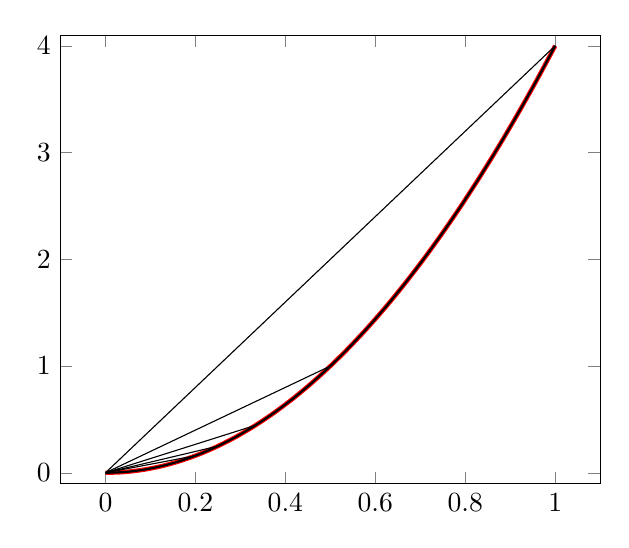
\begin{tikzpicture}
        \begin{axis}[ymin=-0.1, ymax=4.1, xmin=-0.1, xmax=1.1]
          \addplot[smooth,color=red,ultra thick,domain=0:1]{(2*x)^2};
          \foreach \n in {1,...,5}
          {
            \addplot[smooth,domain=0:(1/(\n))]{\n*x*(2/\n)^2};
          }
          \addplot[smooth,color=black,thick,domain=0:1]{(2*x)^2};
        \end{axis}
      \end{tikzpicture}
      \caption{ Een illustratie van de situatie voor $f(x) = x^{2}$}
    \end{figure}
    \end{itemize}
  \end{proof}
\end{vb}

\subsubsection{De $d_2$-metriek op $C(\interval{0}{1})$}
\label{sec:de-d_2-metriek}

\begin{vb}
  Zij $\interval{a}{b}$ een gesloten begrensd interval, dan is $C(\interval{a}{b})$, uitgerust met de volgende functie als metriek, een metrische ruimte:
  \[ d_{2}:\ C(\interval{a}{b})\times C(\interval{a}{b}) \rightarrow \mathbb{R}^{+}:\ (f,g) \mapsto \sqrt{\int_{a}^{b}|f(x)-g(x)|dx} \]
  \extra{bewijs}
  Hint uit de les: het bewijs reduceert zich tot dit:
  \[ \left|\int_{a}^{b}f(x)g(x)\right| < \left(\int_{a}^{b}f(x)^{2}\ dx \right) \left(\int_{a}^{b}g(x)^{2}\ dx \right) \]
  Los hiervoor volgende ongelijkheid uit de genormeerde vectorruimte op met een discriminant.
  \[ \left\| v+\lambda w \right\| > 0 \]
\end{vb}

\begin{st}
  $\forall f,g \in C(\interval{a}{b}):\ d_{1}(f,g) \le d_{\infty}(f,g)$
\extra{bewijs}
\end{st}

\begin{de}
  Noem de verzameling functies $f:\ \mathbb{R} \rightarrow \mathbb{R}$ die in beide oneindigheden naar $0$ gaan: $C_{0}(\mathbb{R})$.
\end{de}

\begin{vb}
  De functie $d$ als volgt, is niet alleen geen metriek voor $C_{0}(\mathbb{R})$, ze is ook niet goed gedefinieerd.
  \[ \int_{-\infty}^{+\infty}|f(x)-g(x)|\ dx \]
  De integraal bestaat immers niet steeds.
\end{vb}

\begin{vb}
  De functie $d$ als volgt, is een metriek voor $C_{0}(\mathbb{R})$.
  \[ d(f,g) = \int_{-\infty}^{+\infty}\frac{|f(x)-g(x)|}{1+x^{2}}\ dx \]
 \extra{bewijs}
\end{vb}


\subsection{Het product van metrische ruimten}
\label{sec:het-product-van}

\extra{product van metrische ruimten}

\subsection{Hausdorffmetriek}
\label{sec:hausdorffmetriek}

\begin{de}
  Voor een niet-lege deelverzameling $A$ van $\mathbb{R}^{p}$ en een $r\in \mathbb{R}^{+}$ definie\"eren we de $r$-omhullende $[A]_{r}$ van $A$ als volgt:
  \[ [A]_{r} = \{r \in \mathbb{R}^{p} \mid \exists a \in A:\ d(x,a) \le r \} \]
  Hierin staat $d$ voor de gewone euclidische metriek.
\end{de}

\begin{de}
  Noteer met $\mathcal{F}$ de verzameling van niet-lege gesloten en begrensde deelverzamelingen van $\mathbb{R}^{p}$.
  \[ \mathcal{F} = \{ A \mid A \subseteq \mathbb{R}^{p}, A \text{ is gesloten en begrensd } \} \]
\end{de}

\begin{de}
  We defini\"eren de \term{Hausdorffafstand} $h(F,G)$ tussen twee deelverzamelingen $F,G \in \mathcal{F}$ als volgt:
  \[ h(F,G) = \inf\{ r\in \mathbb{R}^{+} \mid F \subseteq [G]_{r} \text{ en } G \subseteq [F]_{r} \} \]
\end{de}

\begin{blem}
  \label{lem:omhullenden-in-elkaar}
  Zij $A \subseteq \mathbb{R}^{p}$ en $r,s\in\mathbb{R}^{+}$ met $r\ge s \ge 0$.
  \[ [A]_{s} \subseteq [A]_{r} \]

  \begin{proof}
    Dit volgt meteen uit de definitie:
    Kies een $x\in [A]_{s}$, dan bestaat er een $a\in A$ zodat $d(x,a) \le s$ geldt.
    Omdat $r \ge s$ geldt, geldt ook $d(x,a) \le r$ en dus zit $x$ ook in $[A]_{r}$.
  \end{proof}
\end{blem}

\begin{vb}
  De Hausdorffafstand tussen een (vol) gesloten vierkant en zijn omschreven cirkelschijf is gegeven als $\frac{(\sqrt{2}-1)z}{2}$.
  Hierin is $z$ de zijde van het vierkant.

  \begin{proof}
    Beschouw een vierkant $V$ met zijde $z$ en middelpunt $p\in \mathbb{R}^{2}$.
    Merk op dat de omschreven cirkelschijf $C$ hetzelfde middelpunt en straal $r=\frac{z}{\sqrt{2}}$ heeft.
    \begin{figure}[H]
        \centering
        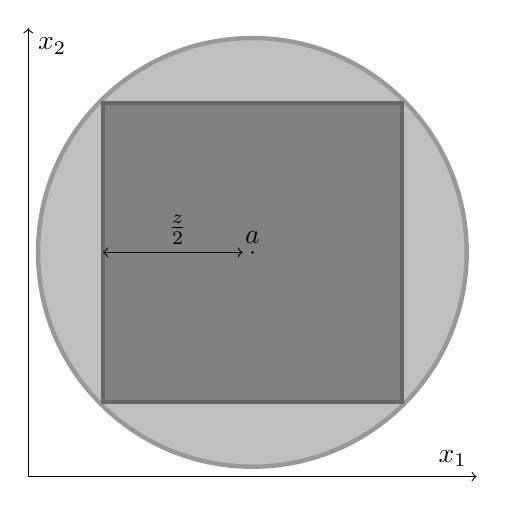
\begin{tikzpicture}
          \begin{axis}[ 
            ticks=none,
            axis lines = middle,
            axis line style={->},
            ymin=0, ymax=3,
            xmin=0, xmax=3,
            xlabel={$x_{1}$},
            ylabel={$x_{2}$},
            axis equal image,
            disabledatascaling
            ]
            \filldraw [ultra thick,fill=black!25!white, draw=black!40!white] (1.5,1.5) circle [radius=sqrt(2)+0.02];
            \filldraw[ultra thick,fill=black!50!white, draw=black!60!white] (0.5,2.5) -- (2.5,2.5) -- (2.5,0.5) -- (0.5,0.5) -- cycle;
            \fill [fill=black] (1.5,1.5) circle [radius=0.01];
            \draw (1.5,1.6) node {$a$};
            \draw (1.5,1.5) node {} edge[<->] (0.5,1.5);
            \draw (1,1.65) node {$\frac{z}{2}$};
          \end{axis}
        \end{tikzpicture}
      \end{figure}
    Voor elke omhullende van de circkel zit het vierkant erin.
    We zoeken dus een de kleinste omhullende van het vierkant dat ook de cirkel omhult.
    Kies $f = \frac{(\sqrt{2}-1)z}{2}$.
    \begin{klad}
      Dit is de afstand tussen een uiterste punt van de cirkel en het dichtstbijzijnde punt op de rand van het vierkant.
      Intu\"itief zou het duidelijk moeten zijn dat dit de Hausdorffaffstand zal zijn.
    \end{klad}
    Beschouw $V_{[f]}$ en kies een willekeurig punt $x$ in de cirkelschijf $C$.
    Er geldt dat $\|x\| < r$ en kies $y = x\frac{\left\|\frac{z}{2}\right\|}{\|r\|}$.
    $y$ ligt dan binnnen $V$\waarom
    Er geldt bovendien:
    \[ \|x-y\| = \|x\| \left|1-\frac{z}{r}\right| \le r - \frac{z}{2} = f \]
    $x$ ligt dus binnen de $f$-omhullende van $V$.
    Er rest ons nog te bewijzen dat $h(C,V)$ zeker niet kleiner is dan $f$.
    Bechouw de rechte door het middelpunt van het vierkant en het midden van een zijde van het vierkant.
    Het is duidelijk dat het dichtste punt $s$ van $C$ tot $V$ het midden $m$ van de zijde van het vierkant is.
    Deze afstand is $f$.
    Als $h(C,V)$ moet dus minstens $f$ bedragen.
  \end{proof}
\end{vb}

\begin{blem}
  Zij $A \subseteq \mathbb{R}^{p}$ en $r,s\in\mathbb{R}^{+}$:
  \[ \left[ [A]_{r}\right]_{s} \subseteq [A]_{r+s} \]

  \begin{proof}
    Kies een $x\in \left[[A]_{r}\right]_{s}$, dan bestaat er een $b\in [A]_{r}$ als volgt:
    \[ d(x,b) \le s \]
    Omdat $b$ in $[A]_{r}$ zit, bestaat er ook een $c\in A$ als volgt:
    \[ d(b,c) \le r \]
    We gebruiken nu de driehoeksongelijkheid:
    \[ d(x,c) \le d(x,b) + d(b,c) \le r + s \]
    $x$ behoort dus tot $[A]_{r+s}$.
  \end{proof}
\end{blem}

\begin{blem}
  Zij $F,G \in \mathcal{F}$ en $r=h(F,G)$.
  \[ F \subseteq [G]_{r} \text{ en } G \subseteq [F]_{r} \]

  \begin{proof}
    Kies een willekeurige $x\in F$.
    Omdat $r = h(F,G)$ geldt, zal volgens de definitie van $h$ het volgende gelden:\lemref{lem:omhullenden-in-elkaar}
    \[ F \subseteq [G]_{r+\frac{1}{n}}\]
    Er bestaat dus een rij punten $(y_{n})_{n}$ in $G$ met de volgende eigenschap:
    \[ \forall n \in \mathbb{N}:\ d(x,y_{n}) \le r + \frac{1}{n} \]
    Omdat $G$ gesloten en begrensd is, bestaat er een deelriij $(y_{n_{k}})_{k}$ die convergeert naar een $y\in G$.\stref{st:in-rp-gesloten-en-begrensd-itv-rijen}
    Voor deze $y$ zal $d(x,y) \le r$ gelden.
    We vinden dus dat $x$ in $[G]_{r}$ zit.
    $F$ moet dus een deel zijn van $[G]_{r}$ en omgekeerd is de redenering hetzelfde met de namen $F$ en $G$ omgewisseld.
  \end{proof}
\end{blem}

\begin{pr}
  De Hausdorffafstand $h$ is een metriek die $\mathcal{F},h$ een metrische ruimte maakt.

  \begin{proof}
    We gaan de eigenschappen van een metrische ruimte na.
    \begin{itemize}
    \item $\forall F,G\in \mathcal{F}:\ h(F,G) \ge 0$: Dit volgt meteen uit de definitie.
    \item $\forall F,G\in \mathcal{F}:\ h(F,G) = 0 \Leftrightarrow F = G$: Idem
    \item $h$ is symmetrisch: Dit zit vervat in de definitie.
    \item $h$ voldoet aan de driehoeksongelijkheid.
      Kies 3 elementen $F$, $G$ en $H$ uit $\mathcal{F}$.
      Noem $s=h(F,G)$ en $t=(G,H)$.
      Meteen vinden we het volgende:
      \[ G \subseteq [H]_{t} \quad\text{ en }\quad F \subseteq [G]_{s} \subseteq \left[[H_{t}]\right]_{s} \subseteq [H_{t+s}] \]
      Analoog vinden we $H \subseteq [F]_{t+s}$ en bijgevolg $h(F,H) \le s+t$.\needed
    \end{itemize}
  \end{proof}
\end{pr}

\begin{opm}
  Het is belangrijk dat de deelverzamelingen waartussen we de afstand meten gesloten en begrensd zijn.
  Stel immers dat \'e\'en ervan niet begrensd zou zijn, dan bestaat de Hausdorffafstand niet.
  Een $r$-omhulling heeft immers een eindige $r$ nodig om zinvel te zijn.
  Stel anderzijds dat de verzamelingen niet gesloten zouden zijn, dan bestaat het supremem in de definitie niet noodzakelijk.
\end{opm}

\begin{st}
  \[ \forall x,y \in \mathbb{R}^{p}:\ h(\{x\},\{y\}) = d(x,y) \]

  \begin{proof}
    
  \end{proof}
\end{st}
\begin{opm}
  We kunnen $\mathbb{R}^{p},d$ dus als deelruimte van $\mathcal{F},h$ via de inbedding $\mathfrak{i}$ als volgt:
  \[ \mathfrak{i}:\ \mathbb{R}^{p} \rightarrow \mathcal{F}:\ x \mapsto \{x\} \]
\end{opm}

\begin{vb}
  Beschouw $F_{1} = B\interval{x_{1}}{r_{1}}$ en $F_{2}= B\interval{x_{2}}{r_{2}}$.

\extra{bewijs: $h(F_{1},F_{2}) = d(x_{1},x_{2}) + |r_{1}-r_{2}|$.}
\end{vb}

\extra{voorbeelden van HDafstandberekeningen}

\begin{st}
  Een rij gesloten bollen $(B_{n})_{n}$ in $\mathbb{R}^{p}$ met middelpunten $x_{n}$ en stralen $r_{n}$ zal voor de Hausdorffmetriek convergeren naar een gesloten bol $B$ met middelpunt $x$ en straal $r$ als en slechts als $\lim_{n\rightarrow +\infty}x_{n}=x$ en $\lim_{n\rightarrow +\infty}r_{n} = r$ gelden.
\extra{bewijs}
\begin{klad}
\begin{proof}
  \begin{lem}
    $\forall r,s \in \mathbb{R}^{+}:\ \left[B\interval{x}{r}\right]_{s} = B\interval{x}{r+s}$
  \end{lem}

  \begin{lem}
    $\forall r\in \mathbb{R}^{+}:\ B\interval{x}{r} \subseteq B\interval{y}{r+\|x-y\|}$
  \end{lem}
  Gevalsonderscheid.
\end{proof}
\end{klad}
\end{st}

\begin{st}
  $(n)_{n}$ in $\mathbb{R}$ is voor de gewone metriek geen Cauchyrij maar wel voor de $d_{2}$-metriek.
\extra{bewijs}
\extra{wat met de $d_1$-metriek?}
\end{st}

\begin{vb}
  Beschouw de niet-lege, gesloten, begrensde deelverzameling $F_{n}$ van $\mathbb{R}$ als volgt voor een $n\in \mathbb{N}_{0}$.
  \[ F_{n} = \{0,1\} \cup \left\{ \frac{i}{n} \ \middle|\ i \in \mathbb{N}, 0 \le \frac{i}{n} \le 1 \right\} \]
  De rij $(F_{n})_{n}$ convergeert volgens de Hausdorffmetriek.
  \begin{proof}
    \begin{klad}
      Om een idee te krijgen van hoe $F_{n}$ eruit ziet tekent u best een paar instanties.
      U ziet dan meteen dat $(F_{n})_{n}$ zal convergeren.

      \begin{figure}[H]
        \centering
        \foreach \n in {1,...,20} {
          \begin{tikzpicture}
            \foreach \l in {0,...,\n} {
              \node(\n\l) at (\l/\n,0) {\textbullet};
            }
          \end{tikzpicture}
        }
      \end{figure}
      Het ziet ernaar uit dat $(F_{n})_{n}$ naar $\interval{0}{1}$ zal convergeren.
      Het kan van pas komen om de Hausdorffafstand van $F_{n}$ tot $\interval{0}{1}$ voor een paar getallen $n\in \mathbb{N}_{0}$ te berekenen.

      \begin{figure}[H]
        \centering
        \foreach \n in {1,...,9} {
          \begin{tikzpicture}
            \foreach \l in {0,...,\n} {
              \fill [thick,fill=black!25!white,opacity=0.2] (\l/\n,) circle [radius=1/(2*\n)];
              \node(\n\l) at (\l/\n,) {\textbullet};
            }
          \end{tikzpicture}
        }
      \end{figure}
      \[
      \begin{array}{|c|c|c|c|c|c|c|c|}
        \hline
        n & 1 & 2 & 3 & 4 & 5 & 6 & i\\
        \hline
        H(F_{n},L) & \frac{1}{2} & \frac{1}{4} & \frac{1}{6} & \frac{1}{8} & \frac{1}{10} & \frac{1}{12} & \frac{1}{2i}\\
        \hline
      \end{array}
      \]
      Vanaf de derde $F_{n}$ zou het patroon duidelijk moeten zijn.
    \end{klad}
    Merk op dat de Hausdorffafstand tussen $F_{n}$, voor een gegeven $n\in \mathbb{N}_{0}$ en $\interval{0}{1}$ steeds $\frac{1}{2n}$ meet.
    Kies willekeurig een $\epsilon \in \mathbb{R}_{0}^{+}$ en noem $n_{0}= \frac{1}{2\epsilon}$.
    Kies nu willekeurig een $n\in\mathbb{N}$,strikt groter dan $n_{0}$.
    \[ h(F_{n},\interval{0}{1}) = \frac{1}{2n} < \frac{1}{2n_{0}} = \frac{2\epsilon}{2} = \epsilon \]
    $(F_{n})_{n}$ convergeert dus naar $\interval{0}{1}$ voor de Hausdorffmetriek.
  \end{proof}
\end{vb}

\begin{vb}
  \label{vb:ttt-2-2014-1}
  \examenvraag{TTT II 2014}
  Beschouw de niet-lege, gesloten, begrensde, deelverzameling $F_{n}$ van $\mathbb{R}^{2}$ als volgt voor een $n\in \mathbb{N}_{0}$.
  \[ F_{n} = \left\{ \left(\frac{k}{n},\frac{t}{n}\right) \middle| t,k \in \{0,\dotsc,n\} \right\} \]
  De rij $(F_{n})_{n}$ convergeert volgens de Hausdorffmetriek.

  \begin{proof}
    Merk op dat we inderdaad over de Hausdorffafstand kunnen spreken omdat de $F_{n}$ niet leeg, gesloten en begrensd zijn.
    \begin{klad}
      Om een idee te krijgen van hoe $F_{n}$ eruit ziet zal u waarschijnlijk minstens twee intanties ervan moeten tekenen.
      Wanneer we die verzamelingen tekenen krijgen we een idee van de convergentie van $F_{n}$ en bovendien van de limiet.

      \begin{figure}[H]
        \centering
        \foreach \n in {1,...,20} {
          \begin{tikzpicture}
            \foreach \k in {0,...,\n} {
              \foreach \l in {0,...,\n} {
                \node(\n\k\l) at (\k/\n,\l/\n) {\textbullet};
              }
            }
          \end{tikzpicture}
        }
      \end{figure}
      Het ziet ernaar uit dat de limiet er als volgt zal uitzien:
      \[ L = \{ (x,y) \mid x,y\in\interval{0}{1} \} \]
      Het kan van pas komen om de Hausdorffafstand van $F_{n}$ tot $L$ voor een paar getallen $n\in \mathbb{N}_{0}$ te berekenen.

      \begin{figure}[H]
        \centering
        \foreach \n in {1,...,9} {
          \begin{tikzpicture}
            \foreach \k in {0,...,\n} {
              \foreach \l in {0,...,\n} {
                \fill [thick,fill=black!25!white,opacity=0.2] (\k/\n,\l/\n) circle [radius=sqrt(2)/(2*\n)];
                \node(\n\k\l) at (\k/\n,\l/\n) {\textbullet};
              }
            }
          \end{tikzpicture}
        }
      \end{figure}
      \[
      \begin{array}{|c|c|c|c|c|c|c|c|}
        \hline
        n & 1 & 2 & 3 & 4 & 5 & 6 & i\\
        \hline
        H(F_{n},L) & \frac{\sqrt{2}}{2} & \frac{\sqrt{2}}{4} & \frac{\sqrt{2}}{6} & \frac{\sqrt{2}}{8} & \frac{\sqrt{2}}{10} & \frac{\sqrt{2}}{12} & \frac{\sqrt{2}}{2i}\\
        \hline
      \end{array}
      \]
    \end{klad}
    Merk op dat de Hausdorffafstand tussen $F_{n}$, voor een gegeven $n\in \mathbb{N}_{0}$, en de verzameling $L$ als volgt steeds $\frac{\sqrt{2}}{2n}$ meet.
    \[ L = \{ (x,y) \mid x,y\in\interval{0}{1} \} \]
    Kies willekeurig een $\epsilon \in \mathbb{R}_{0}^{+}$ en noem $n_{0} = \frac{1}{\sqrt{2}\epsilon}$.
    Kies nu willekeurig een $n\in \mathbb{N}$, strikt groter dan $n_{0}$.
    \[ h(F_{n},L) = \frac{\sqrt{2}}{2n} < \frac{\sqrt{2}}{2n_{0}} = \frac{\sqrt{2}^{2}\epsilon}{2} = \epsilon \]
    $(F_{n})_{n}$ convergeert dus naar $L$ voor de Hausdorff metriek.
  \end{proof}
\end{vb}

\begin{opm}
  Het patroon van de twee bovenstaande voorbeelden kunnen we voorzetten naar $\mathbb{R}^{p}$.
  Daar is de Hausdorffafstand tussen $F_{n}$ en $L$ dan $\frac{\sqrt{p}}{2n}$ en convergeert $(F_{n})_{n}$ naar een $p$-dimensionale gesloten cubus.
\end{opm}

\end{document}

%%% Local Variables:
%%% mode: latex
%%% TeX-master: t
%%% End:
